\documentclass[12pt]{article}
\usepackage{algorithmicx}
\usepackage[ruled]{algorithm}
\usepackage{algpseudocode}
\usepackage{algpascal}
\usepackage{algc}
\usepackage{url,enumerate, amssymb, anysize, booktabs, amsfonts}
\usepackage[colorlinks = true,
linkcolor = blue,
urlcolor  = blue,
citecolor = green,
anchorcolor = blue]{hyperref}
\usepackage{setspace,listings}
\usepackage[dvipdfmx]{graphicx}
\usepackage{amsmath}
\usepackage{psfrag}
\usepackage[font=small,labelfont=bf]{caption}
\usepackage{enumerate}
\usepackage{natbib}
\usepackage{url} % not crucial - just used below for the URL 


\begin{document}
	
	\title{Outline of \\``Testing independence between networks and nodal attributes via multiscale metrics''}
	
	\author{Youjin Lee}
	
	\maketitle
		
%%%%%%%%%%%%%%%%%%%%%%%%%%%%%%%%%	
\subsection*{1. Introducing network topology}

\begin{figure}[H]
	\centering
	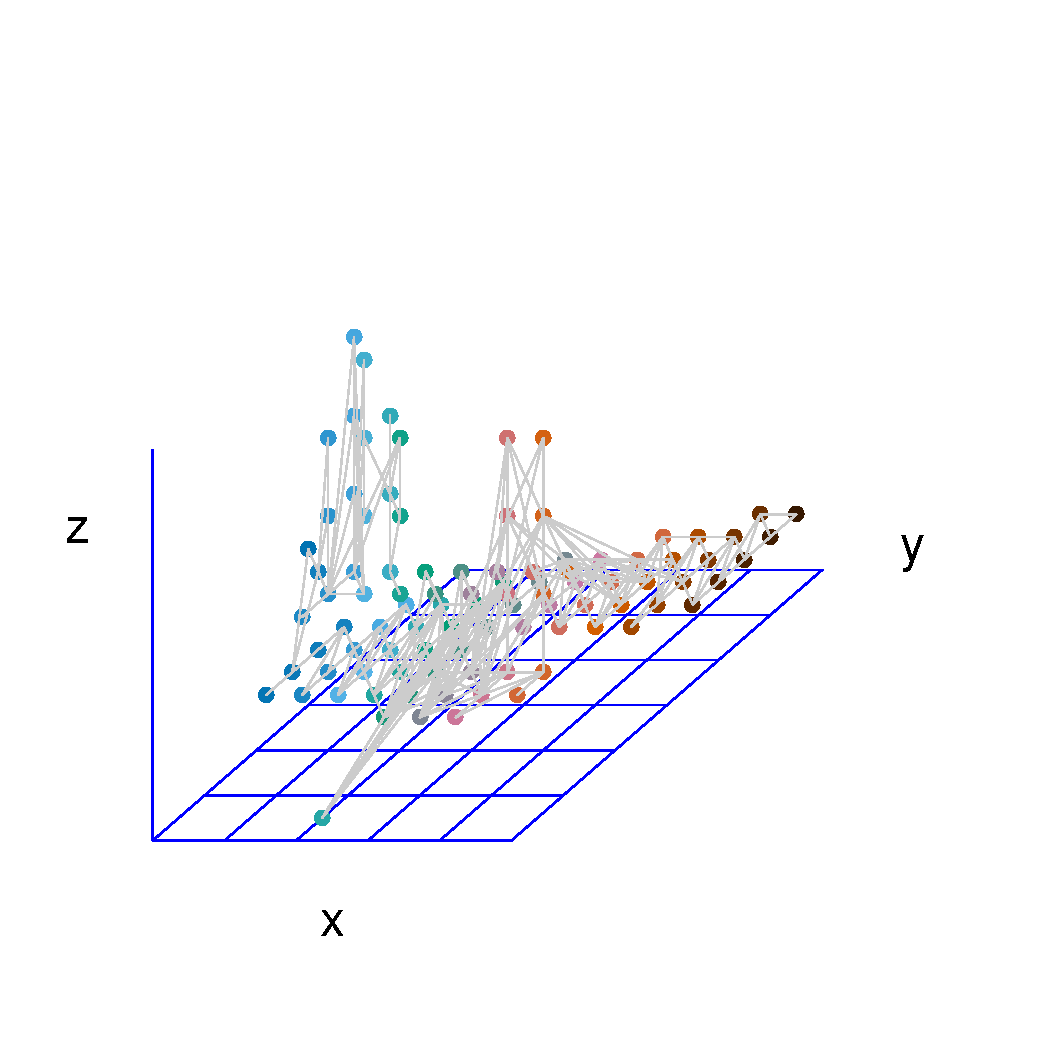
\includegraphics[width=2in]{../Figure/intro.pdf}	
	\caption{Physical location of one component of human brain network and its tracts that connect one vertex to another.}
	\label{fig:intro}
\end{figure}

We introduce a concept of each node's location over their underlying network to bring up the problem of testing independence between distance in terms of network in distance-based test. 


\subsection*{2. Multiscale Generalized Correlation}

\begin{figure}[H]
	\centering
	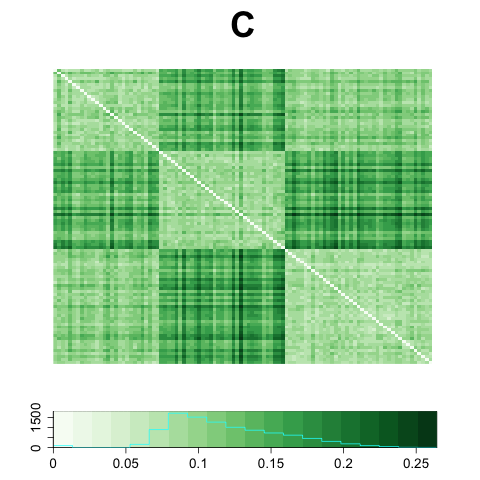
\includegraphics[width=1.5in]{../Figure/C.png}
	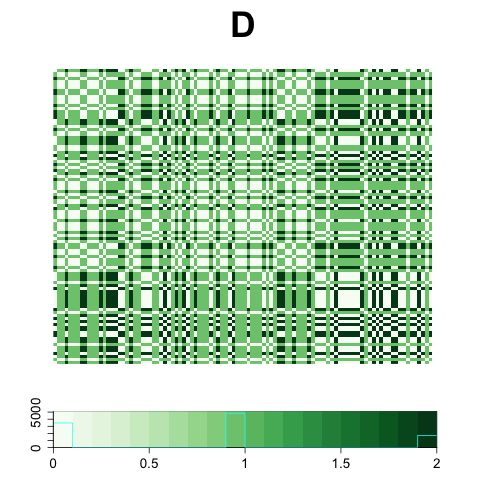
\includegraphics[width=1.5in]{../Figure/D.png}
	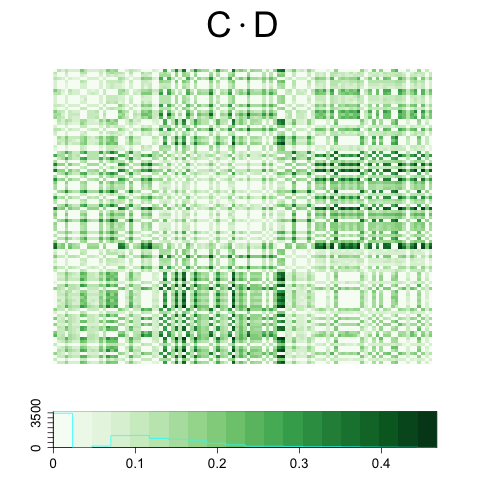
\includegraphics[width=1.5in]{../Figure/CD.png}
	
	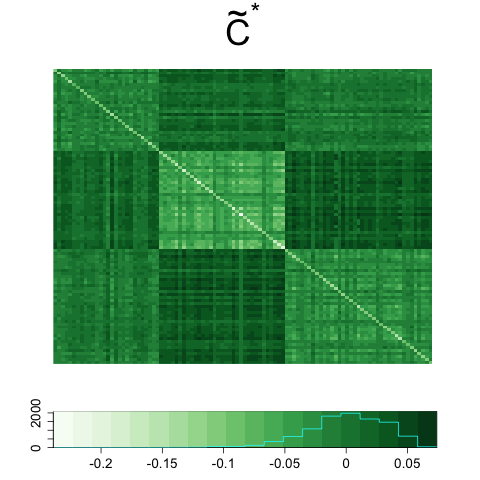
\includegraphics[width=1.5in]{../Figure/tildeCtrunc.png}
	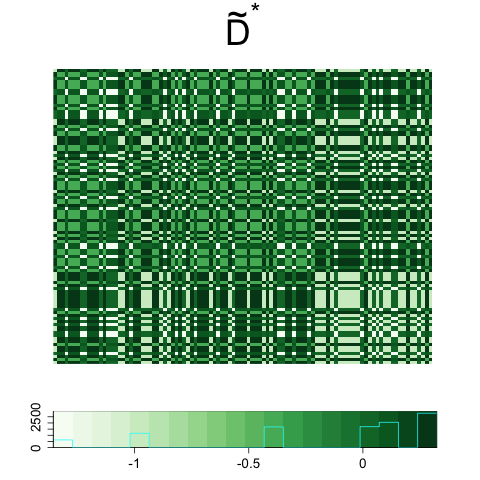
\includegraphics[width=1.5in]{../Figure/tildeDtrunc.png}
	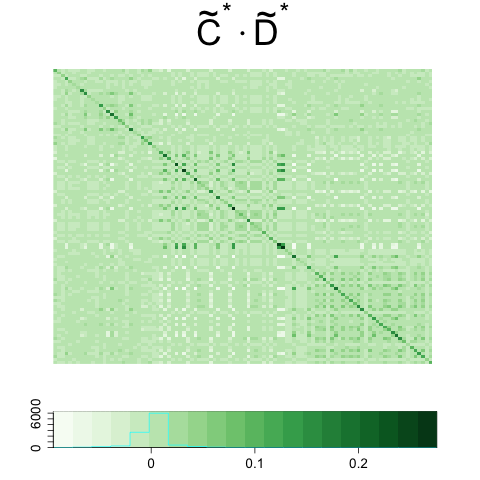
\includegraphics[width=1.5in]{../Figure/tildeCDtrunc.png}
	\caption{(a) Top : Euclidean distance of diffusion maps at time $t=3$, $C$; Euclidean distance of $X$, $D$; element-wise product of $C$ and $D$. (b) Bottom : truncated double-centered  $\tilde{C}$ by $k^{*}$th nearest neighbor in $C$; truncated double-centered $\tilde{D}$ by $l^{*}$th nearest neighbor in $D$; element-wise product of two truncated matrices $\tilde{C}^{*}$ and $\tilde{D}^{*}$. }
	\label{fig:MGCmatrices}
\end{figure}	

As an efficient distance-based test in existence of nonlinear dependency and high-dimensionality, we adopt using local scale distance correlation which truncates each component of distance matrices up to a certain rank.

\subsection*{3. Problems in adopting  valid distance metric defined over network}

\begin{figure}[H]
	\centering
	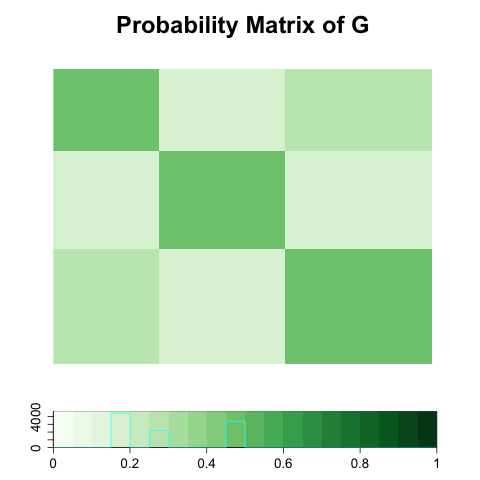
\includegraphics[width=1.5in]{../Figure/pmat.png}
	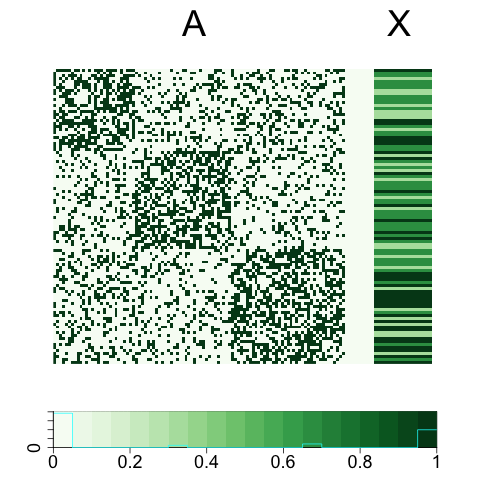
\includegraphics[width=1.5in]{../Figure/Amat.png}
	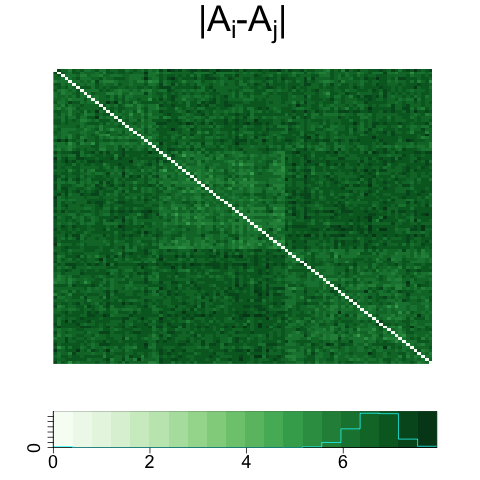
\includegraphics[width=1.5in]{../Figure/distA.png}
	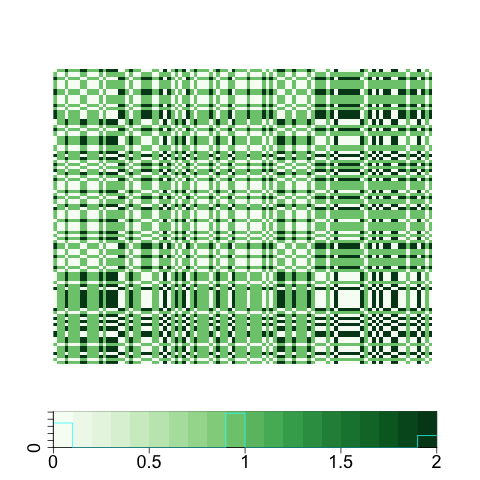
\includegraphics[width=1.5in]{../Figure/distX.png}
	\caption{Population probability distribution and realized values of $A$ and $X$ (scaled by 1/3) in the left two panels. Euclidean distance applied to realized $A$ and $X$ are presented in the right two panels.}
	\label{fig:matrics}
\end{figure}	
  
Every information on edge distribution is denoted in an adjacency matrix so we can consider its Euclidean distance matrix as an ingredient of the test statistics as well as that of nodal attributes.
  
\subsection*{4. demonstrate the validity of diffusion matrix } 

\begin{figure}[H]
	\centering
	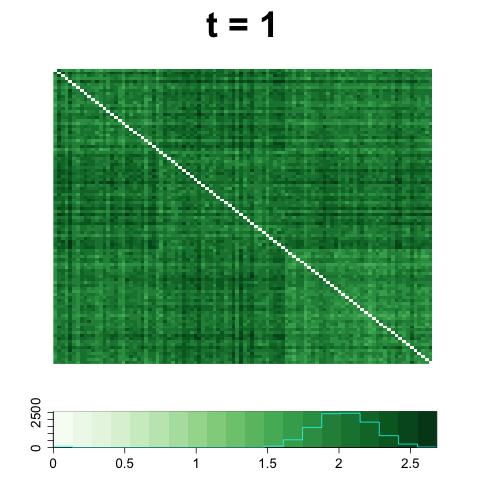
\includegraphics[width=1.5in]{../Figure/Dx1.png}
	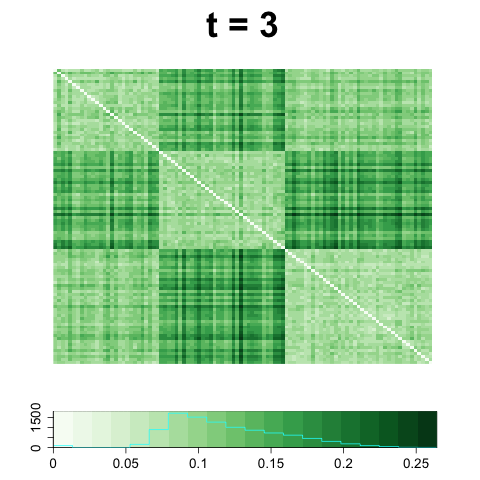
\includegraphics[width=1.5in]{../Figure/Dx3.png}
	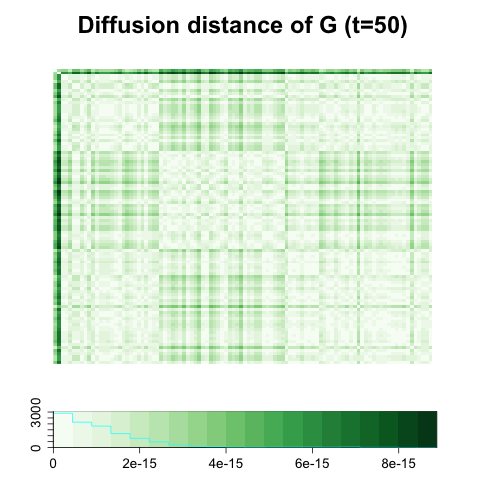
\includegraphics[width=1.5in]{../Figure/Dx50.png}
	\caption{Diffusion distance, i.e. Euclidean distance of diffusion maps at $t=1$, $t=3$  and $t=50$ of sample graph $G$ from Stochastic Block Model.}
	\label{fig:diffusions}
\end{figure}	

Out of concerns on theoretical and also practical shortcomings of using an adjacency matrix, we introduce a one-parameter family of network metrics called \textit{diffusion matrix} which keeps every information of adjacent relation and also effectively captures the clustering of networks. 

\subsection*{5. Introducing the simulation study}

\begin{figure}[H]
	\centering
	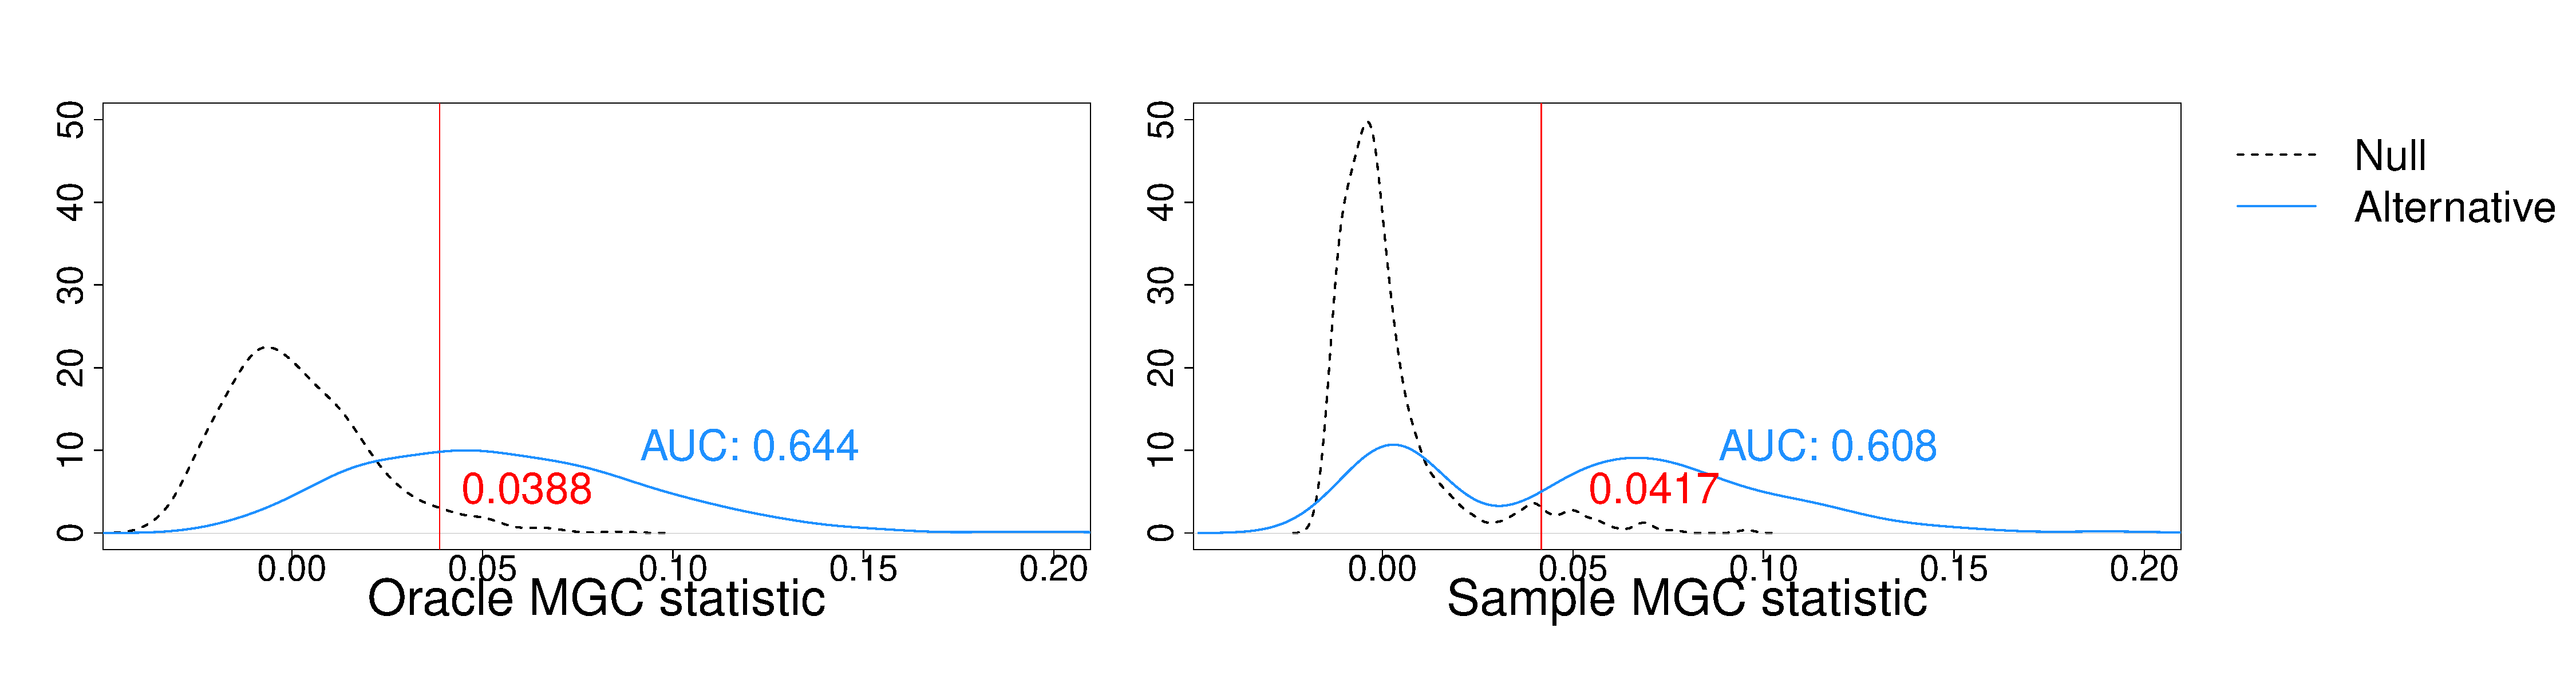
\includegraphics[width=6in]{../Figure/density.pdf}
	\caption{Statistics under null distribution and dependent distribution based on $M = 500$ independently generated SBM with three Blocks}
	\label{fig:density}
\end{figure}	
 
 Throughout the simulation study, we are going to make a comparison between the proposed statistics from null simulated networks and also attribute-dependent simulated networks to calculate the empirical power, based on \texttt{Oracle MGC} and \texttt{Sample MGC}.
 
 
\subsection*{6. Simplest Stochastic Block Model}
 
\begin{figure}[H]
	\centering
	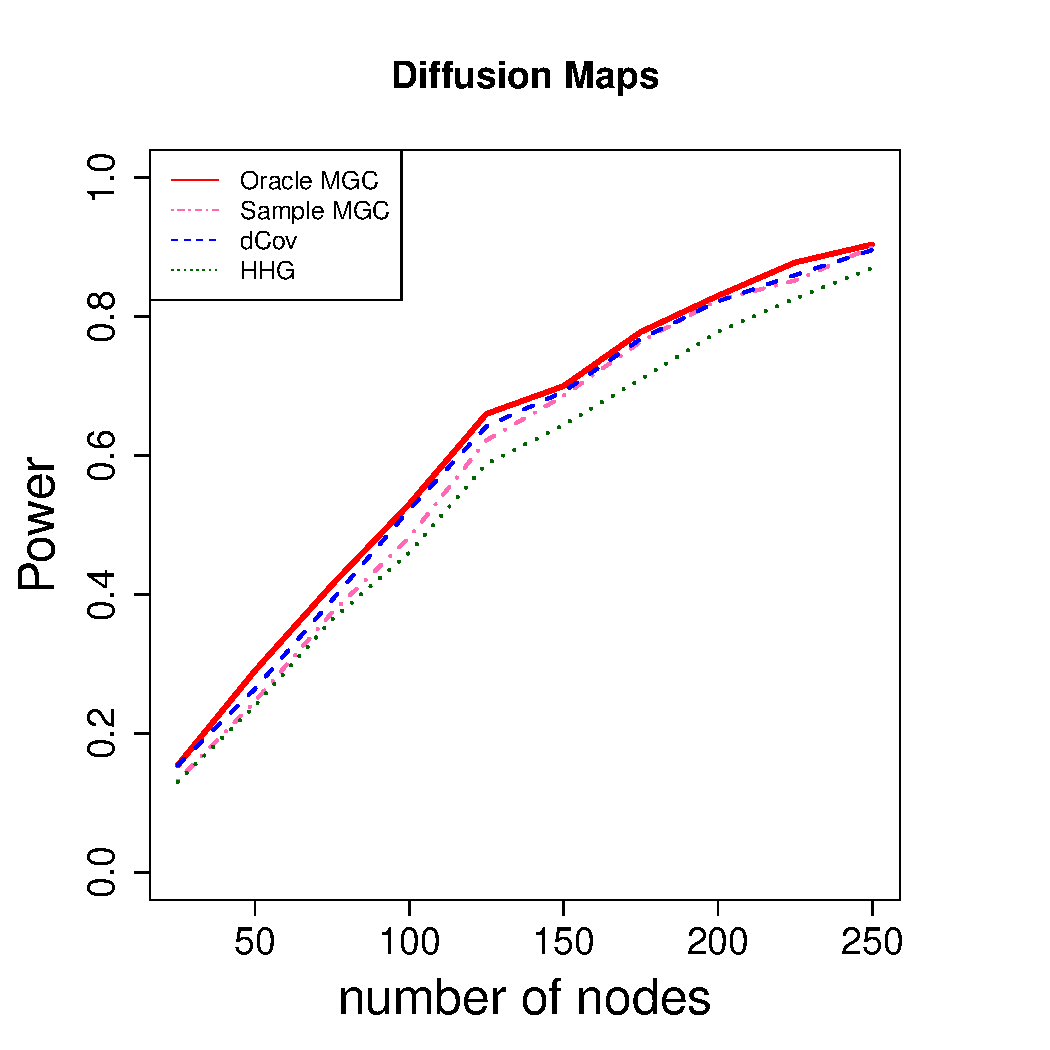
\includegraphics[width=6in]{../Figure/twoSBM.pdf}
	\caption{Empirical power based on $M = 500$ independently generated two-block SBM using diffusion maps (left) and Euclidean of adjacency matrix (middle)  and estimated latent position(right). The most right figure contains the results of \texttt{FH} test as well.}
	\label{fig:twoSBM}
\end{figure}

First simplest SBM with two blocks illustrates the typical case of linear-dependence so that we have similar results for each distance-based tests as well as \texttt{FH}-test.


\subsection*{7. Stochastic Block Model with non-linearly Dependent Attributes}

\begin{figure}[H]
	\centering
	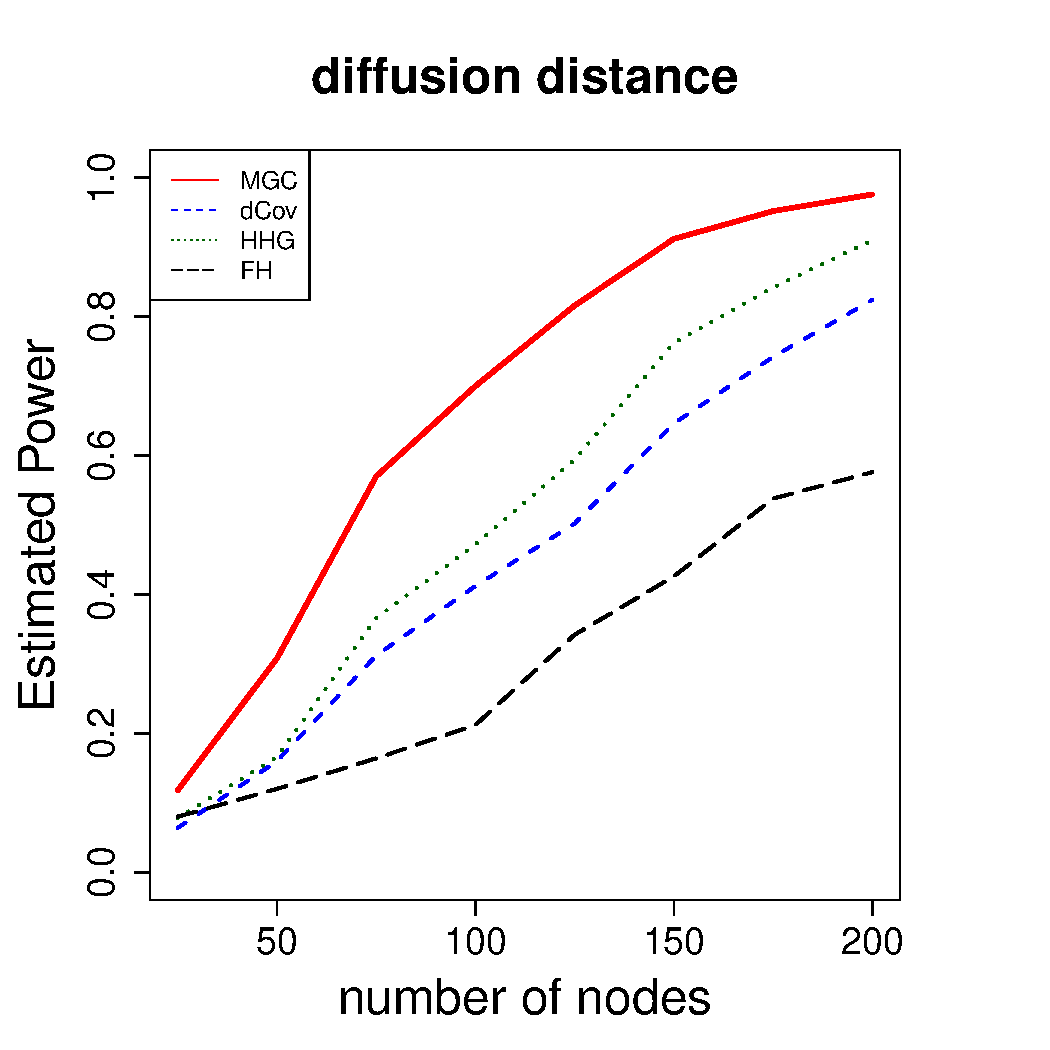
\includegraphics[width=6in]{../Figure/ThreeSBM.pdf}
	\caption{Empirical power based on $M = 500$ independently generated three-block SBM using diffusion maps (left) and Euclidean of adjacency matrix (middle)  and estimated latent position(right). The most right figure contains the results of \texttt{FH} test as well.}
	\label{fig:Three}
\end{figure}	

Next SBM is our punch line that \texttt{MGC} shows its superiority over other statistics especially in diffusion maps metrics and also results higher power in estimated latent position metric than \texttt{FH}.

\subsection*{8. Superiority of the proposed method under non-linear dependency}

\begin{figure}[H]
	\centering
	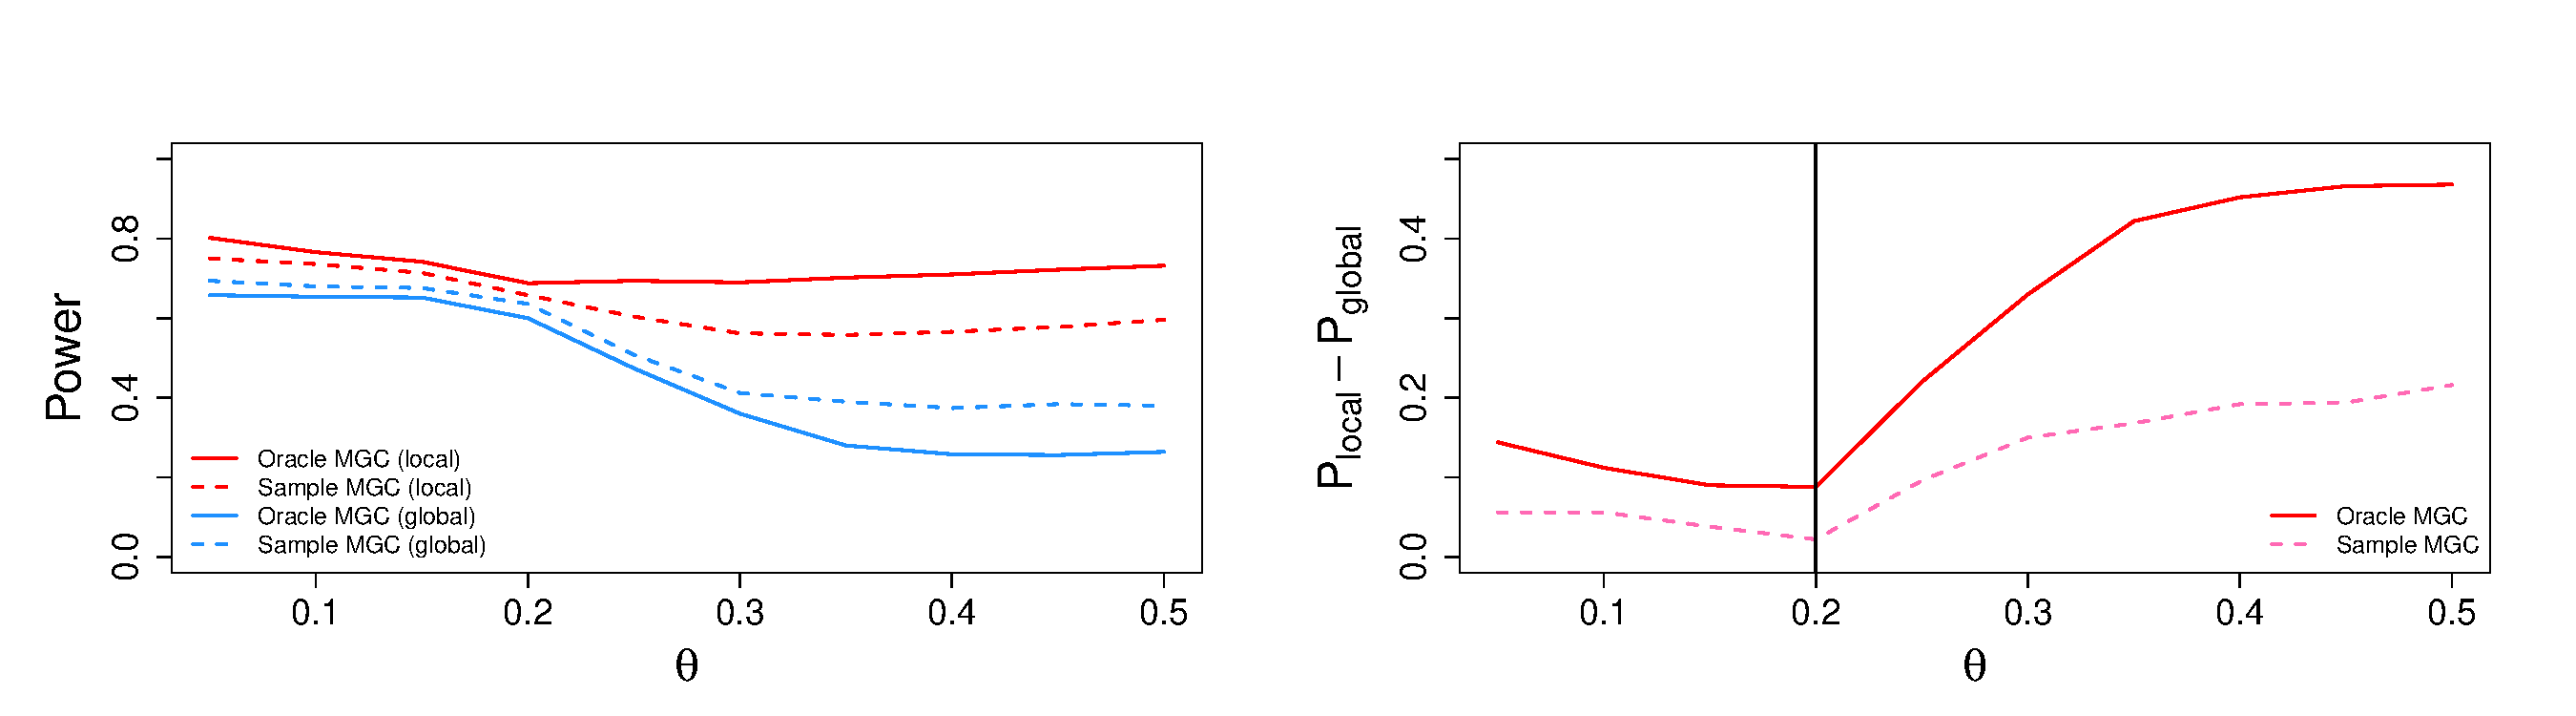
\includegraphics[width=5in]{../Figure/powerplot.pdf}
	\caption{Change of empirical power across $\theta$ in both local and global scale of distance correlation (left). Change of difference between these two powers in Oracle and Sample \texttt{MGC}. Superiority of optimal local scale become evident from $\theta > 0.2$, when distribution of edges have non-linear dependence on $X$.}
	\label{fig:powerplot}
\end{figure}

This plot deeps into when exactly our proposed tests exerts better performance; in the existence of non-linearity which can be formalized into conditional distribution of $A_{ij}$ given Euclidean distance between $\mathbf{X}_{i}$ and $\mathbf{X}_{j}$.

\subsection*{9. Degree-corrected SBM with increased variability in node distribution}	

\begin{figure}[H]
	\centering
	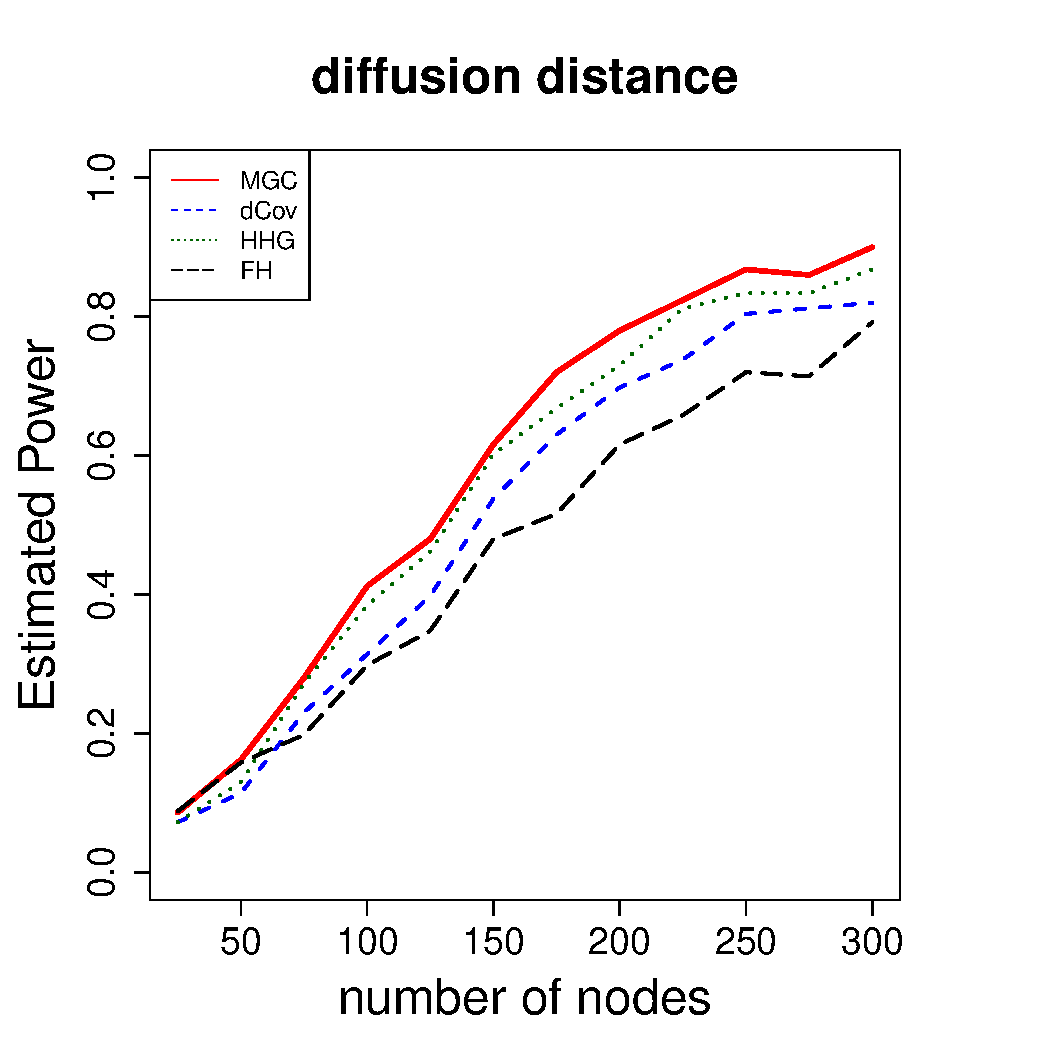
\includegraphics[width=6in]{../Figure/dcSBM.pdf}
	\caption{Empirical power based on $M = 500$ independently generated degree-corrected SBM using diffusion maps (left) and Euclidean of adjacency matrix (middle)  and estimated latent position(right). The most right figure contains the results of \texttt{FH} test as well.}
	\label{fig:dcSBM}
\end{figure}	

Since previous two SBMs might not demonstrate the real example, we introduce a SBM but with increase variability in edge distribution and especially claim the improved power of diffusion maps when variance in an adjacency matrix is relatively higher.



\subsection*{10. Validity of the method even under competitor's model}

\begin{figure}[H]
	\centering
	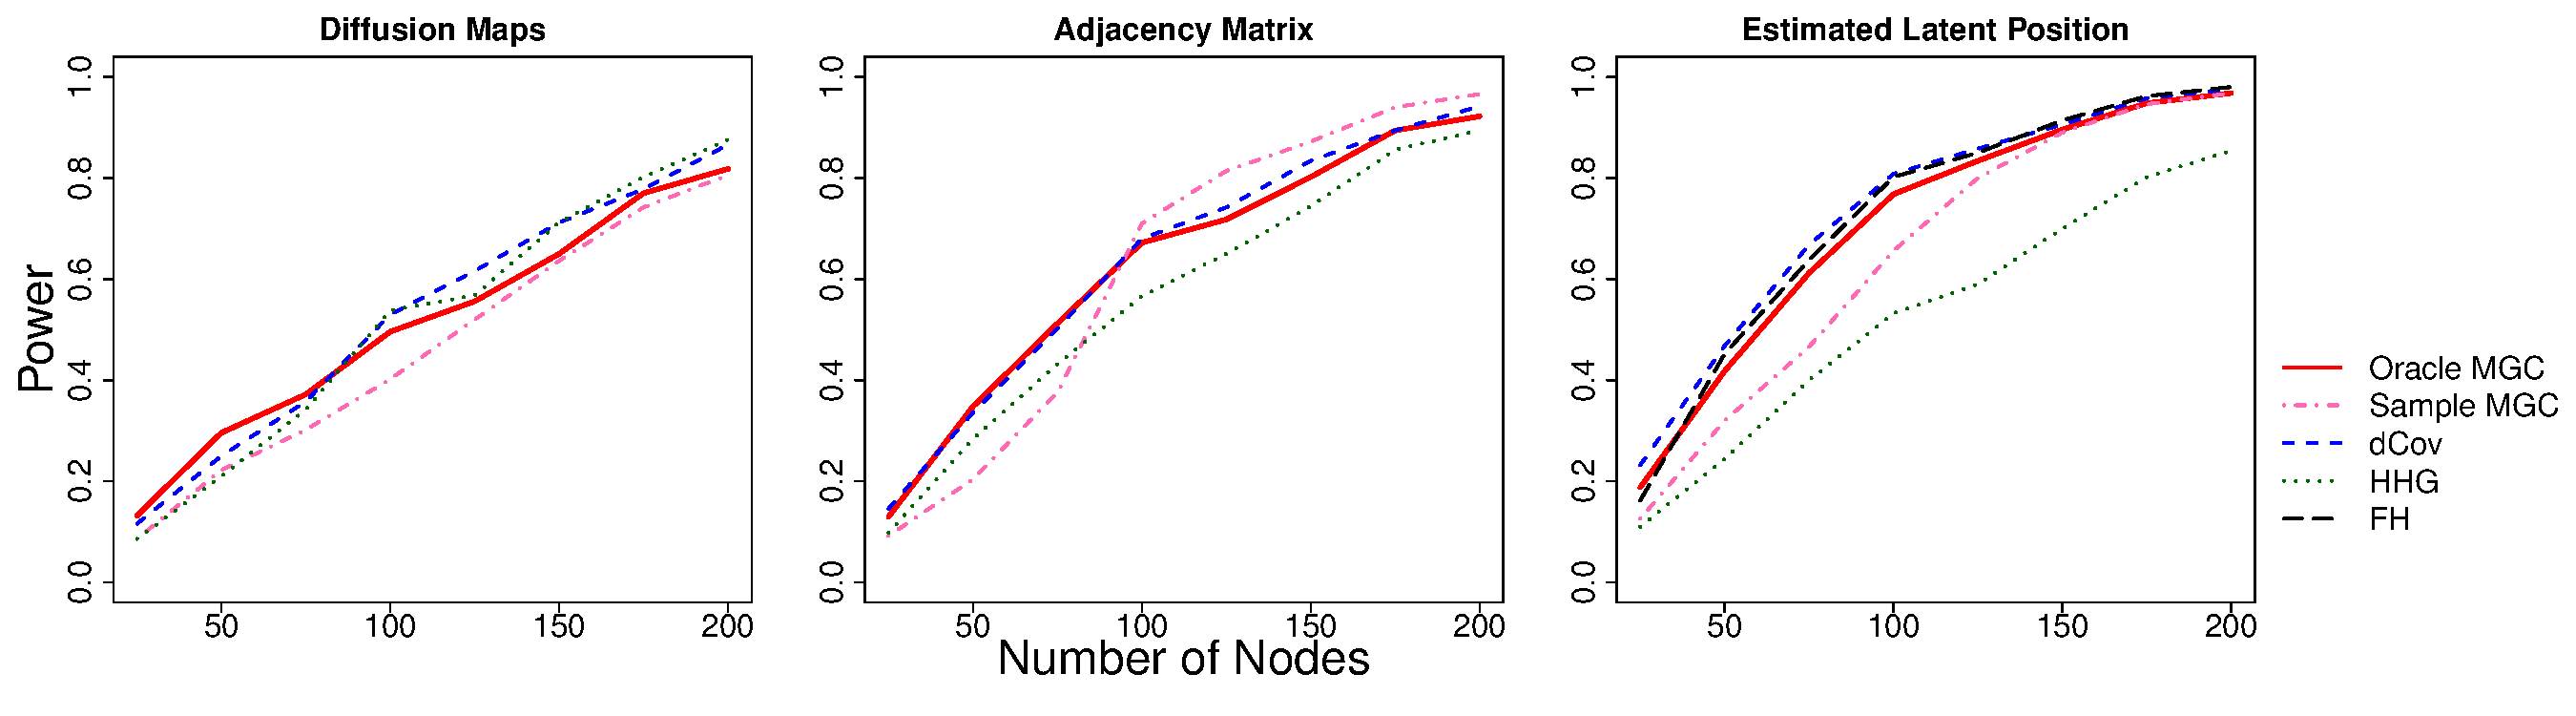
\includegraphics[width=6in]{../Figure/ame.pdf}
	\caption{Empirical power based on $M = 500$ independently generated additive and multiplicative graph model using diffusion maps (left) and Euclidean of adjacency matrix (middle)  and estimated latent position(right). The most right figure contains the results of \texttt{FH} test as well.}
	\label{fig:ame}
\end{figure}	

However it would be fair to include others' mode-based tests and we can still suggest using estimated latent factors when the model is correct; but within that metrics our method does as good as their method. 

\subsection*{11. Node Contribution}

\textcolor{red}{Include one plot which shows validity of our measure of node-specific contribution to the tests.}




\end{document}